\subsection{Work process}
The work process (see examples in \autoref{fig:kanban} and \autoref{fig:backcast}) consisted of weekly sprints, starting with a group meeting on Monday, before the supervisor meeting the same day. At the group meeting, the back-casting was reviewed, and an overview of the week's tasks was provided via the kanban board. Then the tasks were discussed and delegated in small groups, often consisting of two people working together. To manage both the kanban board and the back-cast timeline, we utilized the GitHub projects feaature. 
The development process was iterative, allowing continuous refinement of both hardware and software components. Early prototypes were tested and evaluated, and feedback from these tests informed subsequent design decisions. This approach ensured that potential technical challenges were identified early and that system functionality evolved in alignment with the project requirements.

\begin{figure}[H]
    \centering
    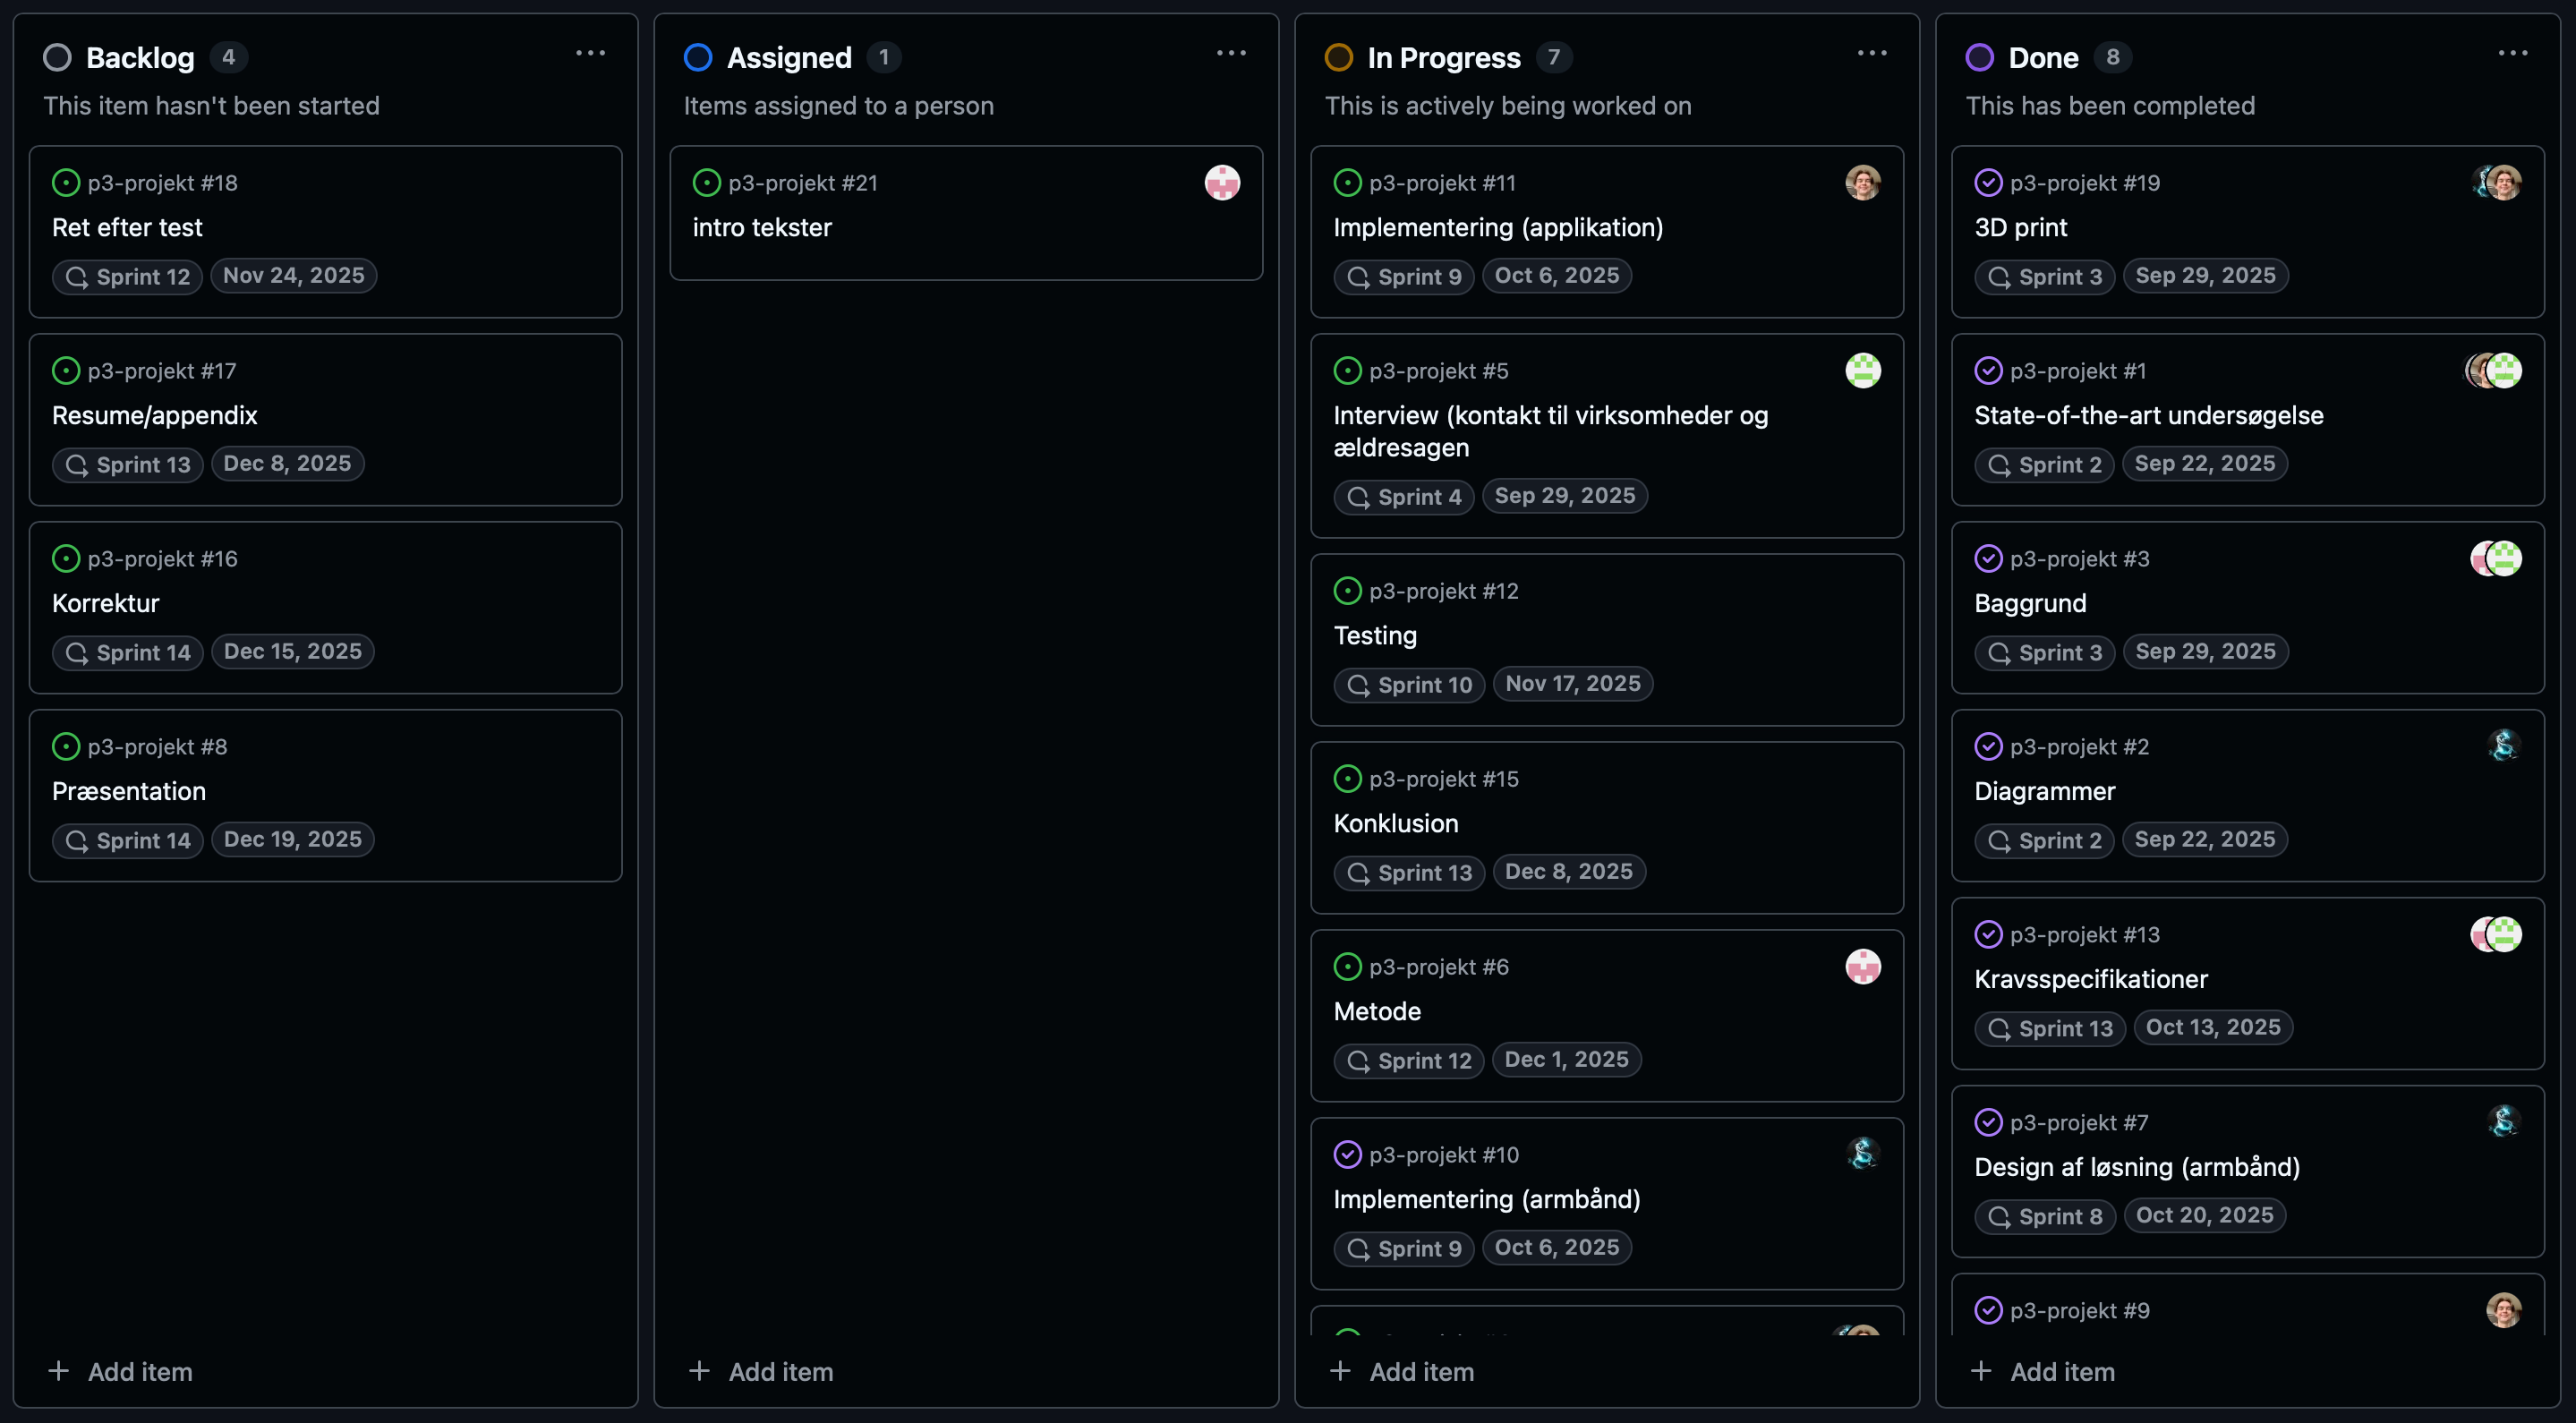
\includegraphics[width=0.75\linewidth]{report/images/Kanban.png}
    \caption{Kanban board}
    \label{fig:kanban}
\end{figure}

\begin{figure}[H]
    \centering
    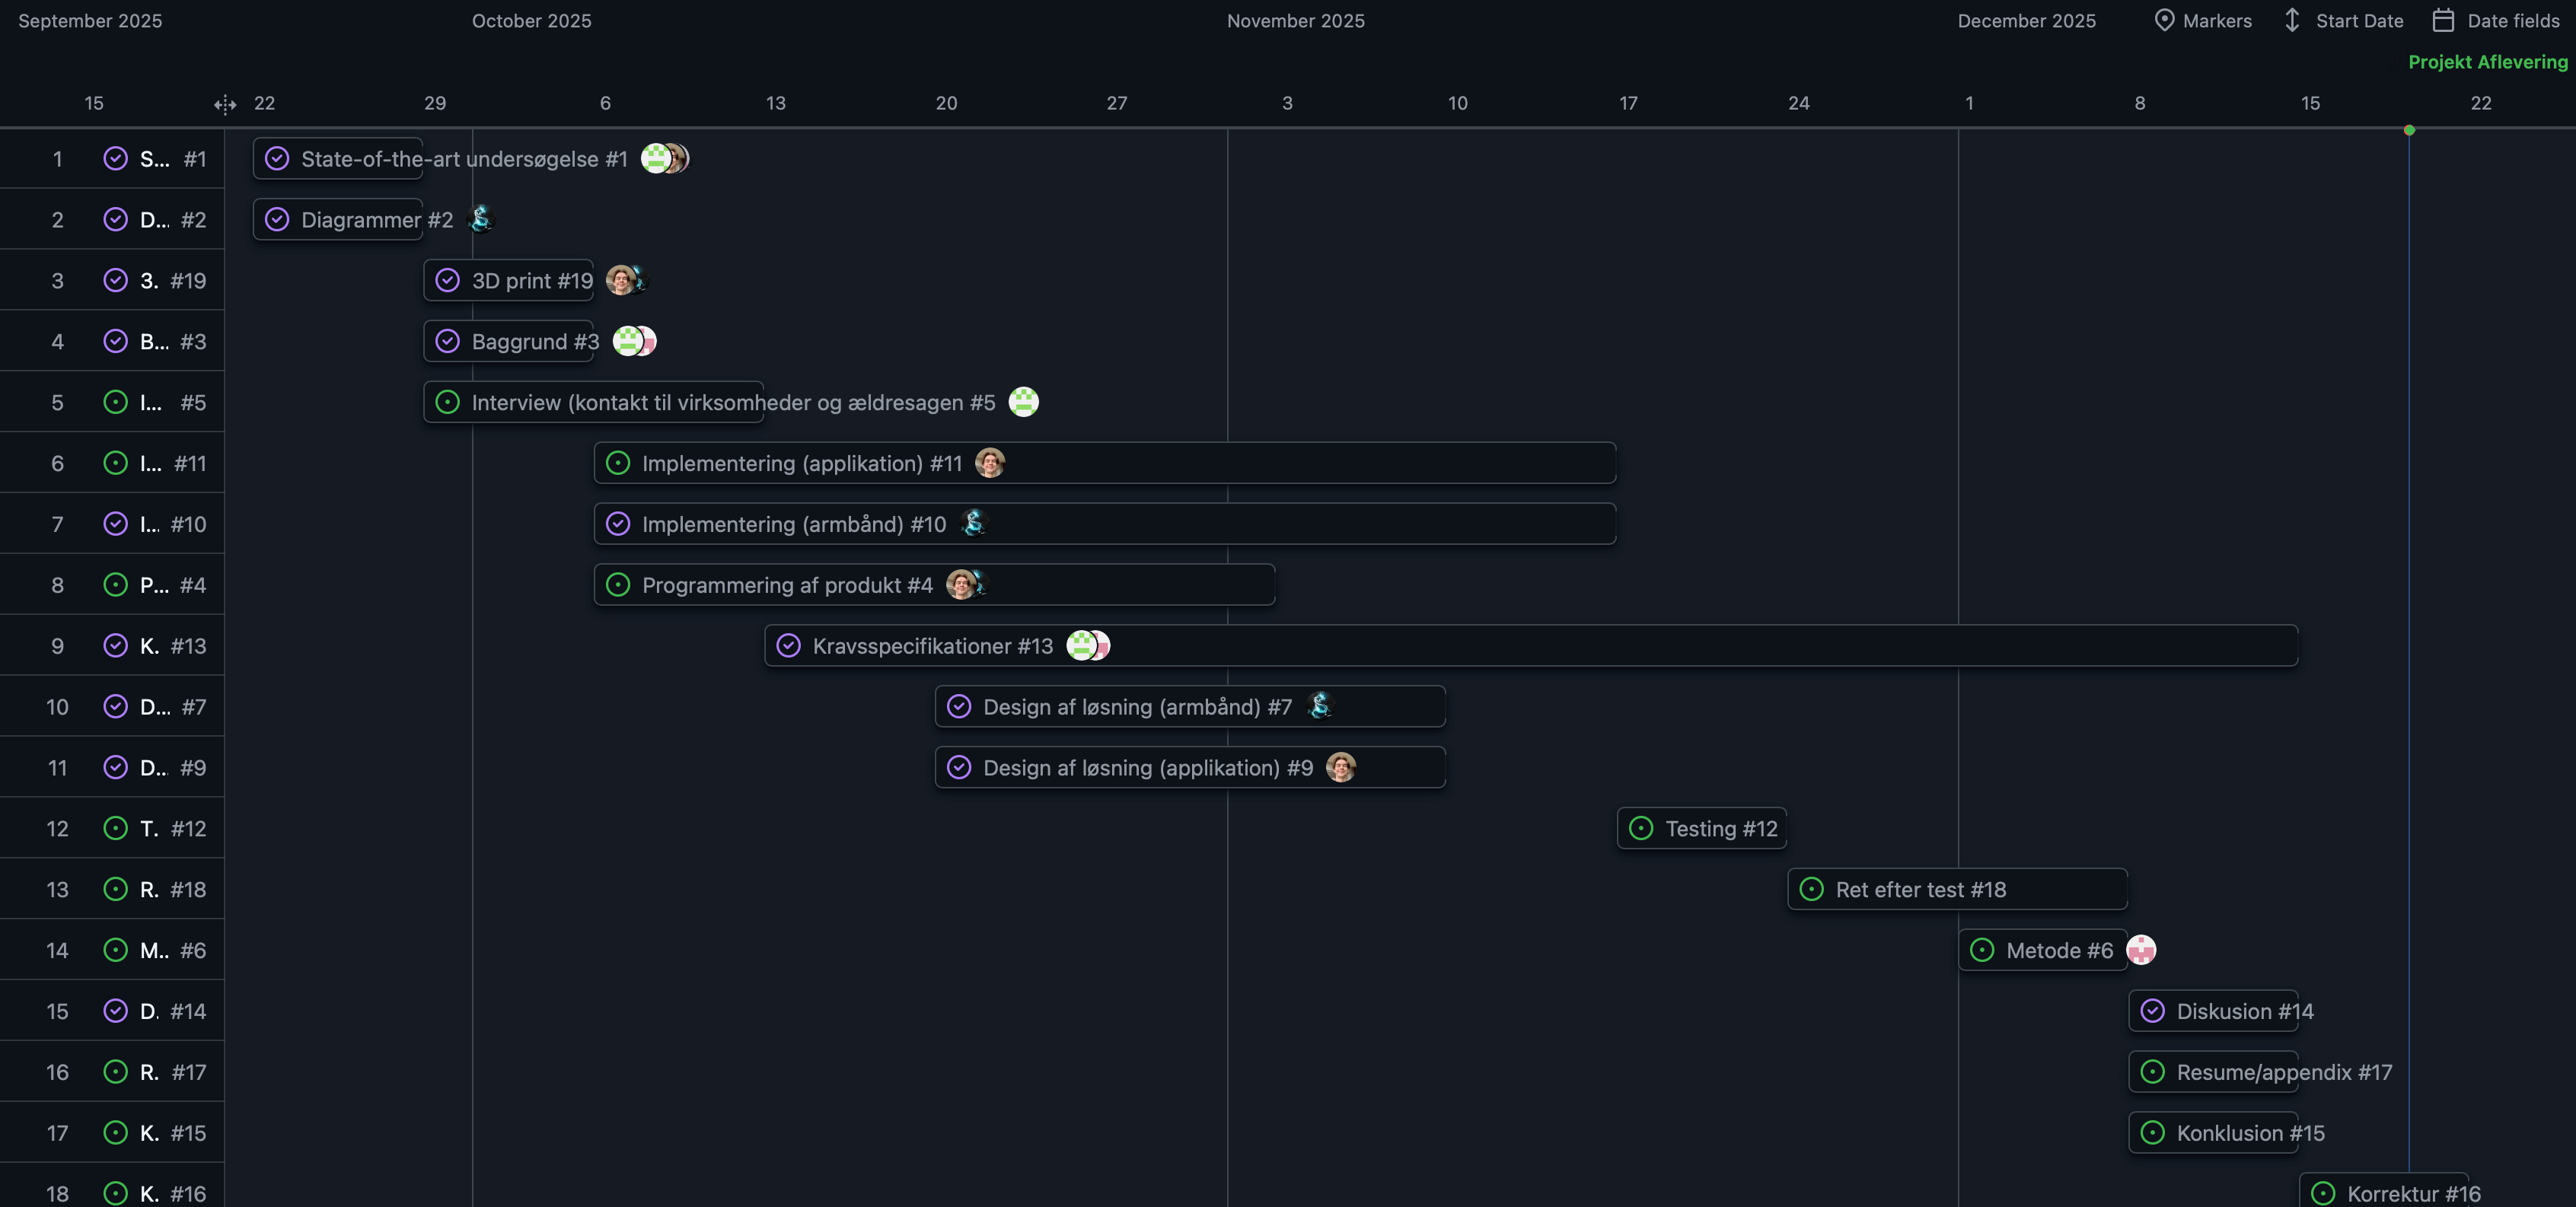
\includegraphics[width=0.75\linewidth]{report/images/Backcast.png}
    \caption{Backcast}
    \label{fig:backcast}
\end{figure}

\subsection{Background}
The  methodology for the introduction began with the search \textit{ældrebyrden i Danmark} (the burden of the elderly in Denmark). After that, Ældresagens databases \textit{Analyser og undersøgelser om ældre} and \textit{Ældre i tal} (elderly people in numbers) was found. The following keywords were used to search for further articles and statistics: \textit{demografi}, \textit{hjemmehjælp og rehabilitering}, \textit{dagligdag}, \textit{pårørende}, \textit{sundhedsvæsen og velfærdsteknologi} (demography, domiciliary care and rehabilitation,everyday life, relatives, healthcare and welfare technology). Furthermore the group was sent some articles from Ældresagen in a mail regarding a possible interview; these were picked by a consultant at Ældresagen. 

